
%%% Latex preamble
\documentclass[11pt]{article}
\oddsidemargin 0pt
\textwidth 6.5in
\topmargin -0.65in
\textheight 9.25in

\usepackage{epsfig}
\usepackage{natbib}
\usepackage{amssymb}
%Get the citation punctuation correct
\bibpunct{(}{)}{;}{a}{}{,}

%Set the space between paragraphs.
%Uncomment this for single spacing, comment for double spacing
\setlength{\parskip}{1.0ex plus0.5ex minus0.2ex}

%Allow colour in your output (pdf only?)
% \usepackage[usenames,dvipsnames,svgnames,table]{xcolor}
% \definecolor{darkgreen}{rgb}{0,.5,0}	%For example
%%%End of preamble

\newcommand{\Plwr}{\ensuremath{P_{\mathrm{lwr}}}}
\newcommand{\Pupr}{\ensuremath{P_{\mathrm{upr}}}}


\begin{document}
\begin{center}
\begin{Huge} Some notes on the Box Least Squared Algorithm \end{Huge}
\end{center}

This document describes some notes on my implementation of the BLS.

\section{Choosing the optimal trial periods}

Consider a transit with period $P$ and duration $\tau$ observed continuously
for a timespan $T$. We would expect, on average, to observe $n = T/P$ transits.
Fold this lightcurve on a period $P'$. $P'$ is ``close enough" to $P$ to find the transit if
all points in transit are folded on top of each other (i.e have the same phase) in the folded lightcurve. For simplicity, we will assume that two points have the same phase if their phase differs by less than a transit duration.

Let the phase of the 0th transit is $t0$. The worst error will be on the nth transit (assuming for simplicity that $P$ and $P'$ are close enough that no wrapping in phase occurs. The phase of the $n^{\mathrm{th}}$ transit will be $t0 + n(P-P')$,  where  phase is defined to run from [0..$P$) not, say, [0, 2$\pi$).

If we want all the transits to line up, we require
$$
n(P-P') < \tau
$$

But $n = T/P$, so our requirement that all transits overlap implies 
$$
(P-P') < \tau P/T
$$
%dP := (P-P') < tau \times P/T

Following Kovacs, we will call $\tau/T$ the fractional transit duration, $q$.
To do a blind search where at least one trial period is close enough
to any transit period present, we select periods

\noindent
\Plwr\\
\Plwr\ + (P-P') $= \Plwr + q \Plwr = \Plwr \times (1+q)$\\
\Plwr\ $\times (1+q)^2$\\
...\\
\Plwr\ $\times (1+q)^N$\\

\noindent
(This is considerably fewer steps than \Plwr + $Nq$ steps.)

Now, this will ensure that all transit centres lie within one transit
duration of each other in at least one folded lightcurve. However, this phase difference will still smear out the event quite a bit, making it harder to detect. So we pick an overresolution factor, $R$ to
ensure even better preformance.. Setting $R=2$ ensures
all transit centres lie within half a transit duration of each other. We redefine $q$ such that
$q = \tau/(RT)$

So how many steps, $N$, do we need to get from some \Plwr\ to some other \Pupr?

\begin{eqnarray*}
\Pupr = \Plwr(1+q)^N\\
\Rightarrow \Pupr/\Plwr = (1+q)^N\\
\Rightarrow \log_{(1+q)} (\Pupr/\Plwr) = N\\
\vspace{1ex}\\
\Rightarrow N = \frac{\ln(\Pupr/\Plwr)}{ \ln(1+q)}
\end{eqnarray*}


\section{Computational Cost}
The computational cost is driven by the number of periods searched, $N$, and time taken to bin the data. The binning time is O(n), i.e it scales linearly with the number of input points. The number of periods searched depends on the ratio of the longest and shortest period, and the assumed fractional transit duration, $q$ (i.e transit duration divided by orbital period). $N$ doubles for each factor of $e$ the period span increases. It also scales as $10^{1/q}$. For example, if $q= 0.01$, $100 \times \ln(\Pupr/\Plwr)$ periods are searched. For coding simplicity, $q$ is computed once for the shortest duration and longest period and used for all other periods. This is computationally quite inefficient, but it makes the meaning of the output much simpler. If a faster algorithm is needed, $N$ can be recomputed for each transit duration.


\begin{figure}[bht]
     \begin{center}
    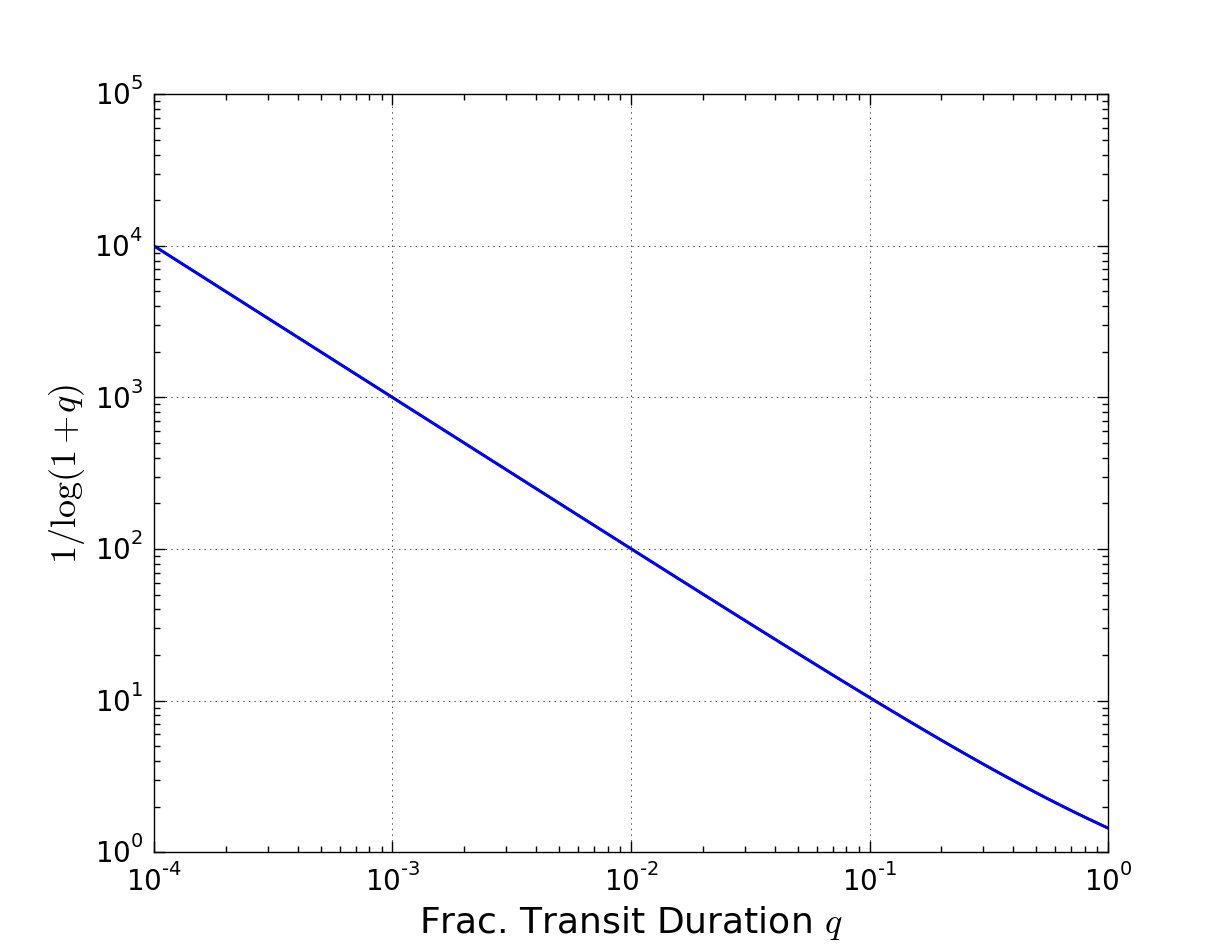
\includegraphics[angle=0, scale=.4]{qplot}
    \caption{Number density of periods searched as a function of assumed fractional transit duration. The actual number of periods searched depends on the ratio between the longest and shortest periods searched.}
     \end{center}
 \end{figure}


\end{document}
